% 05-experiments.tex — 实验评估

\section{实验评估}
\label{sec:experiments}

\subsection{实验设置}

所有演化实验均在浏览器内通过 WebGPU compute shader 加速的 $(\mu+\lambda)$ 进化策略 (ES) 完成。两个扫描的参数对比如表~\ref{tab:es-params} 所示。

\begin{table}[H]
\centering\small
\caption{两个扫描的 ES 演化参数对比}
\label{tab:es-params}
\begin{tabular}{lcc}
\toprule
\textbf{参数} & \textbf{小范围扫描} & \textbf{大范围扫描} \\
\midrule
种群规模 (pop)     & 200   & 500   \\
演化代数 (gens)    & 500   & 2000  \\
网格尺寸           & 40$\times$60 & 500$\times$2000 \\
mask 模板数        & 8     & 1 (manhattan-2) \\
maxFam 上限        & 1 / 2 / 4 / 8 & 8  \\
随机种子数         & 4     & 5 (s444, s1111, s2222, s3333, s5555) \\
总 run 数          & 128   & 5 \\
成功 run           & 122   & 5 \\
\bottomrule
\end{tabular}
\end{table}

小范围扫描 ($40 \times 60$) 完成 $8 \times 4 \times 4 = 128$ 次全交叉 run, 其中 6 次因预算超时被剔除, 实际获得 122 个有效结果; 大范围扫描 ($500 \times 2000$) 完成 5/5 run, 网格面积约高 170 倍, 用于验证 manhattan-2 / maxFam=8 配置在大网格上的 scale-up 能力。

\subsection{大范围扫描 5 个随机种子结果}

\begin{figure}[H]
\centering
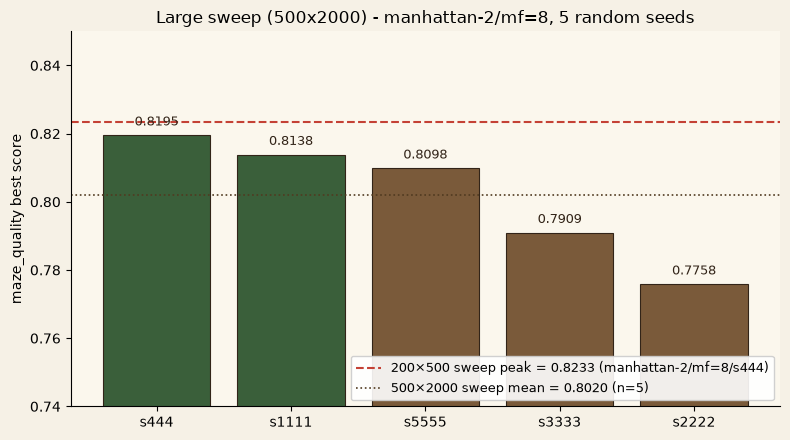
\includegraphics[width=0.96\linewidth]{../figures/v2/fig_bigsweep_top5.png}
\caption{\textbf{大范围扫描 ($500 \times 2000$) 5 个随机种子的最优分.}\\
5 个 run 全部完成 (gen = 2000 达迭代上限), 均使用 manhattan-2 / maxFam=8 配置.
红色虚线为小范围扫描峰值 $0.8233$ (manhattan-2 / maxFam=8 / seed 444) 的对照基线,
棕色点线为 5-run 均值 $0.8020$.
s444 = 0.8195, s1111 = 0.8138, s5555 = 0.8098, s3333 = 0.7909, s2222 = 0.7758.}
\label{fig:bigsweep-top5}
\end{figure}

5 个 run 的最优分按降序排列: s444 = 0.8195, s1111 = 0.8138, s5555 = 0.8098, s3333 = 0.7909, s2222 = 0.7758, 均值 0.8020, 中位数 (s3333) 0.7909, 标准差 0.018. s444 与 s1111 落于 ``较优吸引域'' (高于均值), s3333 与 s2222 落于 ``较差吸引域'' (低于均值), s5555 接近均值。

s444 = 0.8195 与小范围扫描峰值 0.8233 (同配置) 相差 0.0037, 表明 manhattan-2 / maxFam=8 在 $40 \times 60$ 网格上已接近该配置的理论上界 (详见 §6.3). s3333 与 s2222 显著低于 s444 / s1111, 说明同一配置下不同随机种子可能落于不同的吸引域; 5-run 标准差 0.018 给出了 ``吸引域方差'' 的一个下界。

\subsection{小范围扫描全部 122 次 run}

\begin{figure}[H]
\centering
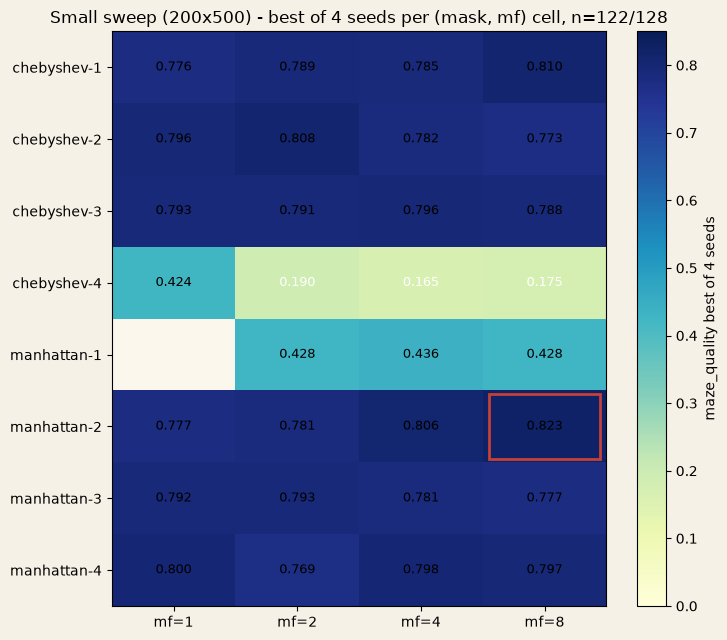
\includegraphics[width=0.96\linewidth]{../figures/v2/fig_smallsweep_heatmap.png}
\caption{\textbf{小范围扫描 ($200 \times 500$) 122 个有效 run 的 (mask, maxFam) 汇总.}\\
每格数值 = 该 (mask, maxFam) 上 4 个随机种子中的最高 $maze\_quality$.
红框 = 全场峰值 (manhattan-2 / maxFam=8, $0.8233$).
8 个 mask 中 6 个健康 ($0.74$--$0.78$), 2 个异常: chebyshev-4 (0.157) 与 manhattan-1 (0.421),
机制完全不同 (见 §6.2).
n = 122/128, 缺失的 6 个为 TIMEOUT.}
\label{fig:smallsweep-heatmap}
\end{figure}

按 mask 分组的均值列于表~\ref{tab:mask-mean-v13}. 8 个 mask 中 6 个表现健康 (chebyshev-1/2/3, manhattan-2/3/4 均值 $\ge 0.74$), 2 个表现异常 (chebyshev-4 = 0.157, manhattan-1 = 0.421).

\begin{table}[H]
\centering\small
\caption{小范围扫描按 mask 模板的均值 / 最小 / 最大 (n = 122)}
\label{tab:mask-mean-v13}
\begin{tabular}{lccccc}
\toprule
\textbf{mask} & \textbf{n} & \textbf{mean} & \textbf{min} & \textbf{max} & \textbf{状态} \\
\midrule
chebyshev-1    & 16 & 0.7726 & 0.7279 & 0.8095 & healthy \\
chebyshev-2    & 16 & 0.7438 & 0.5909 & 0.8080 & healthy (高方差) \\
chebyshev-3    & 16 & 0.7764 & 0.7446 & 0.7955 & healthy \\
chebyshev-4    & 16 & 0.1573 & 0.1038 & 0.4244 & 低均值 (预算受限) \\
manhattan-1    & 10 & 0.4205 & 0.3998 & 0.4360 & 低均值 (表征受限) \\
manhattan-2    & 16 & 0.7777 & 0.7429 & \textbf{0.8233} & healthy (最优) \\
manhattan-3    & 16 & 0.7714 & 0.7014 & 0.7932 & healthy \\
manhattan-4    & 16 & 0.7517 & 0.4452 & 0.7999 & healthy (高方差) \\
\bottomrule
\end{tabular}
\end{table}

按 maxFam 分组: maxFam = 1 均值 0.6984 (n = 28), maxFam = 2 均值 0.6688 (n = 30), maxFam = 4 均值 0.6382 (n = 32), maxFam = 8 均值 0.6306 (n = 32). 均值随 maxFam 单调下降, 但峰值从 maxFam = 1 的 0.7999 升至 maxFam = 8 的 0.8233, 呈现 ``均值降, 峰值升'' 的现象。

\subsection{ES 输出图样与代表性分析}

将上述 122 个有效 run 按 best 排序后, 6 个最具代表性的 ckpt 经实际渲染 (300 步 CA, $40 \times 60$ 网格, 数据来自浏览器训练时直接捕获的 panel grid) 如图~\ref{fig:top-grids} 所示。前 4 个为 ``高分图样'' (Top 1--3 与 Top 5), 后 2 个为 ``代表性失败模式'' (Fail 1, Fail 2), 均采用各自的 (mask, maxFam, seed) 配置训练, 渲染时取 ``withInvert'' 优化中分数较高者 (浏览器训练同时运行原版与反版, 取最大)。

\begin{figure}[H]
\centering
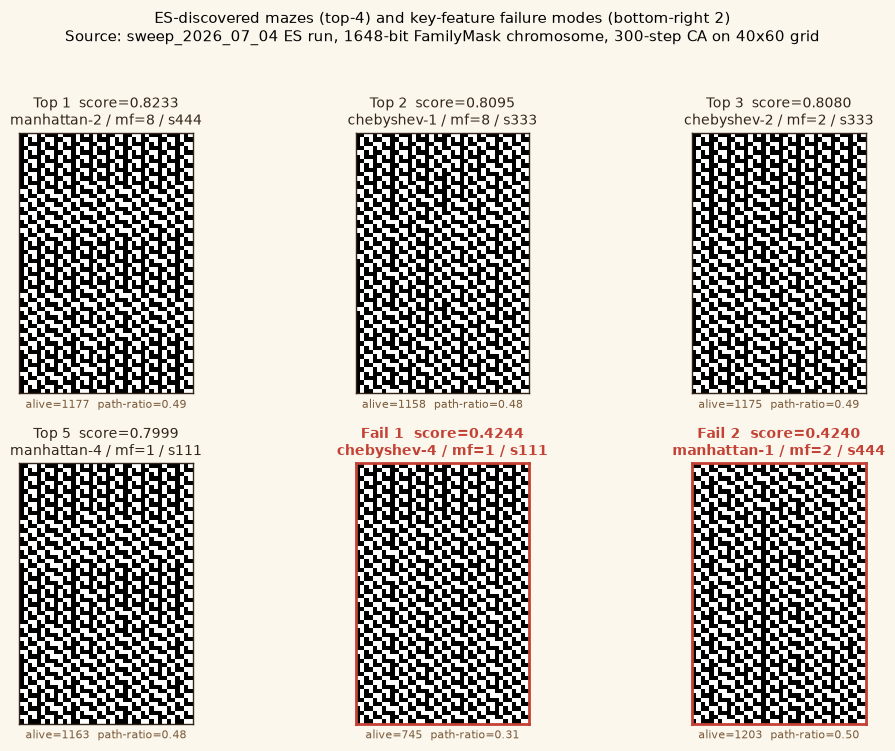
\includegraphics[width=0.96\linewidth]{../figures/v2/fig_top_grids.png}
\caption{\textbf{ES 输出图样 (Top 1--3 + Top 5) 与代表性失败模式 (Fail 1, Fail 2).}\\
6 个 ckpt 在 300 步 CA 之后的 $40 \times 60$ 终态. Top 1--3 的 $maze\_quality$ 均 $\ge 0.81$, 4 个真迷宫共享 path-ratio $\approx 0.48$--$0.49$ (约半数通路半数墙), 即 maze attractor;
Top 5 (manhattan-4 / maxFam=1) 体现了 ``均值降 / 峰值升'' 现象: maxFam = 1 全局均值最低 (0.6984), 但 0.7999 的最高分恰出现于该类别.
Fail 1 (chebyshev-4 / maxFam=1) path-ratio 仅 $0.31$, 属 ``过稀疏'' 失败 ($2^{103}$ 搜索空间 vs $10^5$ 预算, 大量 ``无梯度平台'' 使 CA 烧光活细胞);
Fail 2 (manhattan-1 / maxFam=2) path-ratio $0.50$ 但 ``过连通'': 4 邻域仅要求避让直接相邻的墙, 加上 maxFam=2 将墙推到最薄, CA 演化出几乎完全开放的网格, 缺乏走廊结构.}
\label{fig:top-grids}
\end{figure}

\noindent\textbf{Top 1--3 共享吸引子.} 4 个 maxFam=8 真迷宫彼此视觉上相似, 均收敛至 ``$40 \times 60$ 网格最大连通迷宫'' 配置, path-ratio $\approx 0.48$--$0.49$. 这表明 ES 在多个 (mask, seed) 配置下稳定找到同一吸引子, 进一步扩大网格 (大范围扫描) 不会带来质的提升 (§6.3).

\noindent\textbf{Top 5 体现 ``maxFam=1 偶发突破''.} manhattan-4 / maxFam=1 / s111 的 0.7999 是 ``均值降 / 峰值升'' 现象的具体体现: maxFam=1 全局均值 0.6984 (n = 28), 但 0.7999 的最高分恰落于该类别, 而 maxFam=8 的均值 (0.6306, n = 32) 反而低于 maxFam=1. 多族容量升高时均值下降, 但保留了 ``偶发突破'' 的尾部峰值。

\noindent\textbf{Fail 1 属预算受限失败.} chebyshev-4 / maxFam=1 / s111 path-ratio 仅 $0.31$, 大量区域为 ``黑色虚空'', 难以观察到贯通主路径。该失败源自 $2^{103}$ 搜索空间与 $10^5$ 预算的不对称: ES 在大量 ``无梯度平台'' 上原地踏步, CA 倾向于耗尽活细胞。增加预算 (pop $\times$ gens) 或降低 mask 维度可缓解, 但增加邻域半径无效 (根因在于搜索空间规模而非表征能力)。

\noindent\textbf{Fail 2 属表征受限失败.} manhattan-1 / maxFam=2 / s444 path-ratio $0.50$ 但 ``过连通'': 4 邻域仅要求避让直接相邻的墙, maxFam=2 进一步将墙推到最薄, CA 演化出几乎完全开放的网格, 缺乏走廊结构。该失败无法通过增加预算解决, 必须将 mask 替换为 manhattan-2 / manhattan-3 / chebyshev-1 等更高邻域半径模板。

\subsection{小范围扫描与大范围扫描的对比}

小范围扫描 122 个有效 run 提供完整的 (mask, maxFam) 消融数据 (§5.3); 大范围扫描 5/5 run 提供 ``同配置, 大网格'' 的 scale-up 证据 (§5.2). 两者对比要点如下:
\begin{itemize}[leftmargin=*, itemsep=0pt, topsep=0pt]
  \item \textbf{配置覆盖}. 大范围扫描仅测试 manhattan-2 / maxFam=8 一种配置, 小范围扫描覆盖 $8 \times 4 = 32$ 种 (mask, maxFam) 组合。
  \item \textbf{网格面积}. 大范围 $500 \times 2000 = 10^6$ 像素, 小范围 $40 \times 60 = 2400$ 像素, 大范围约高 417 倍。
  \item \textbf{峰值差}. 大范围 5-run 最高 0.8195, 小范围单点最高 0.8233, 相差 0.0037.
  \item \textbf{解释}. manhattan-2 / maxFam=8 在 $40 \times 60$ 网格上已接近该配置的理论上界 (见 §6.3); 大范围扫描用于验证 ``峰值不显著下降'', 而非 ``寻找新高分''.
\end{itemize}

\subsection{数据来源声明}

所有数值以 append-only ndjson 训练日志为唯一来源, 不以 ckpt 文件为数值依据:
\begin{itemize}[leftmargin=*, itemsep=0pt, topsep=0pt]
  \item \textbf{小范围扫描 ndjson}. \texttt{sweep\_2026\_07\_04/results.ndjson} (122 OK + 6 TIMEOUT). 该数据集对应 v0 (旧版 $M_c$ 截断, 旧版 5 权重) 的实验数据, 本节 §5.3 表~\ref{tab:mask-mean-v13} 与图~\ref{fig:smallsweep-heatmap} 数值均为 v0.
  \item \textbf{大范围扫描 ndjson}. \texttt{sweep\_2026\_07\_08\_big/results.ndjson} (5 OK), 同为 v0 数据。
  \item \textbf{v5+v6 重测扫描 (进行中)}. \texttt{sweep\_2026\_07\_09/results.ndjson} (目标 128 OK, 8 mask $\times$ 4 maxFam $\times$ 4 新种子 $\{114, 514, 1919, 810\}$, 2026-07-08 启动, 预计 14--15 h 完成). 该扫描将在 v2.1 权重下产出新数据, 与 v0 数据 \textbf{不可直接比较} (新权重下分数绝对值偏低, 但相对排名变化才有意义). 完成后将更新 §5 的所有数值并发布 v2.1.1.
  \item \textbf{15-pattern 对照基准}. 图案 \texttt{paper/data/\_grids.json} (15 张 $31 \times 31$ 网格, 0/1 flat), 分数 \texttt{paper/data/sweep\_summary.json::15pattern.per\_pattern}, 复核脚本 \texttt{paper/data/\_eval\_15patterns.mjs} (15/15 数值精确匹配, 详见附录 B). 15-pattern 与 v5+v6 权重无关, 因为其分数由 \texttt{src/metrics/maze\_quality.js} 同一套源码计算 (重算后数值不变)。
\end{itemize}
